\chapter{Introduction}
\setlength{\parskip}{2.5ex plus .4ex minus .4ex}
\section{Sujet de stage}
L'équipe-projet RECORD\footnote{Rénovation et CooRDination de la modélisation de cultures pour la
gestion des agro écosystèmes.} au sein de l'INRA de Toulouse a pour but de développer un logiciel écrit en C++ de modélisation et de simulation des agro-écosystèmes appelé VLE\footnote{Virtual Laboratory Environment}.\\
Ce logiciel modélise des individus grâce au formalisme DEVS\footnote{Discrete Event System Specification}, d'équations différentielles et notamment du plugin Forrester. Ce plugin permet la modélisation d'un individu sous les règles du formalisme de forrester, c'est-à-dire de générer des classes C++ correspondant à la description de l'individu.\\
Ce stage a pour but de faire une extension de ce plugin afin de pouvoir cloner un ou plusieurs individus et permettre à l'utilisateur de prendre des décisions en fonction de l'état du système et/ou du temps qui s'écoule.\\

\section{Contexte}
Ce stage s'inscrit dans mon cursus universitaire pour clôturer ma 4ème année en ingénieurie informatique à Polytech'Nice Sophia.
Durant ce stage, j'ai travaillé de manière indépendante au sein de l'équipe-projet RECORD sur un plugin global du logiciel VLE qui utilise le formalisme DEVS.\\
Ce formalisme est un formalisme modulaire et hiérarchique pour la modélisation, la simulation et l'analyse de systèmes complexes. Il permet de donner une dynamique à un modèle qui peut être amplifiée si celle-ci est déclaré comme exécutive. La différence est que la dynamique prend en considération des évènements en entré, effectue une ou plusieurs actions et renvoye des évènements en sortie au cours du temps alors que l'exécutive peut modifier, créer, supprimer et avoir d'autres actions sur les modèles en plus de toutes les actions réalisées par la dynamique.\\

\begin{minipage}{\linewidth}% to keep image and caption on one page
\makebox[\linewidth]{%        to center the image
  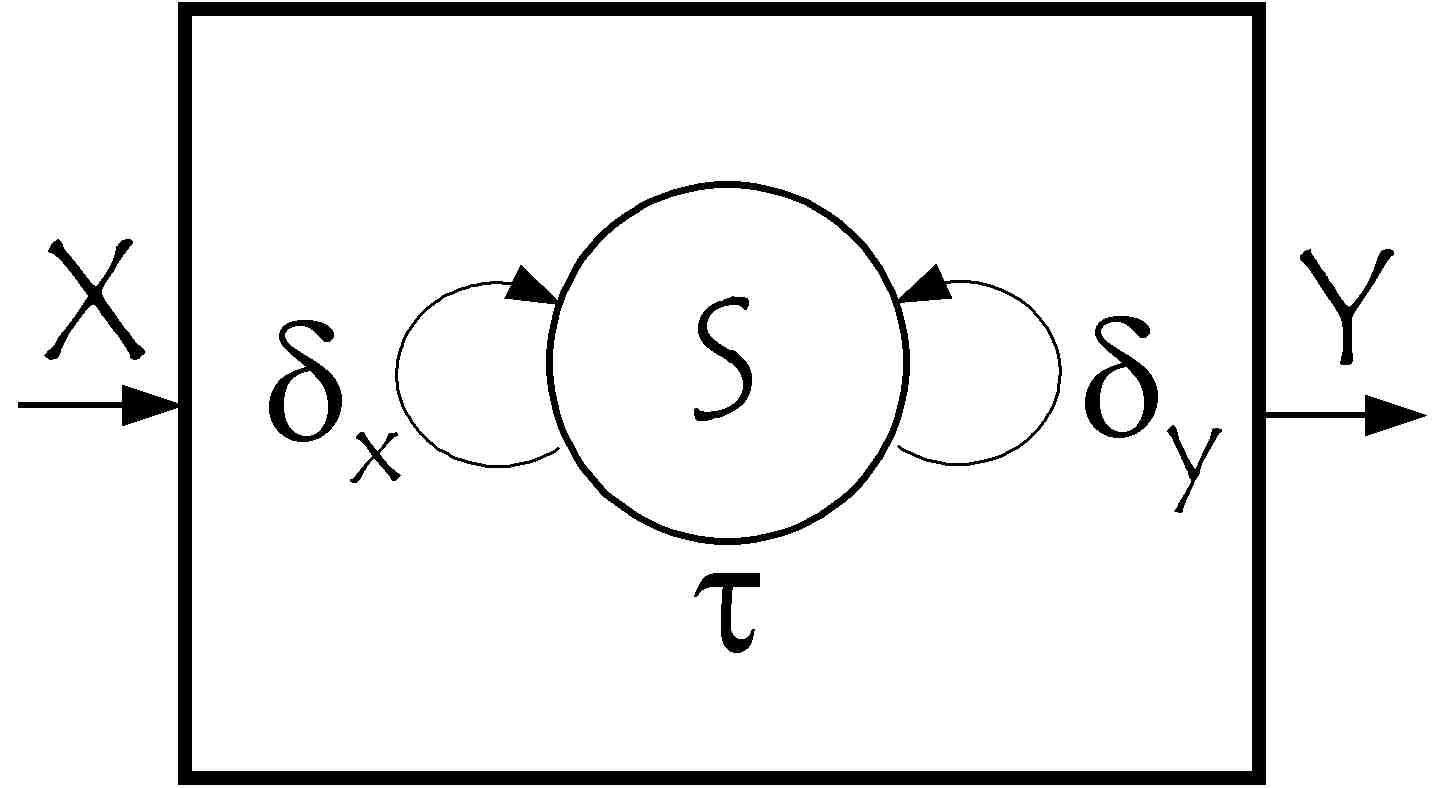
\includegraphics [width=60mm]{images/DEVSPP.jpg}}
\captionof{figure}{Dynamique DEVS}%\label{visina8}%      only if needed  
\end{minipage}

Dans ce schéma représentant le fonctionnement de DEVS, les entrées du modèle sont représentées par X, les sorties par Y, et $\delta_{x}$ la dynamique lors de la réception d'évènement, $\delta_{y}$ la dynamique interne du modèle c'est-à-dire ce qui arrive régulièrement au cours du temps $\tau$. S est l'état du système.
